\chapter{Principi dell'Ingegneria del Software}

Messi in pratica attraverso \textbf{metodologie}, costituite di:
\begin{itemize}
    \item \textbf{Metodi}: linee guida formali che regolano l'esecuzione di attività
    \item \textbf{Tecniche}: approcci di carattere meccanico e con limitata applicabilità
\end{itemize}

\section{Principi}

\paragraph{Rigore e formalità} (o \textit{rigorosità}) Si mantiene un certo livello di rigore per evitare imprecisioni e/o inaccuratezze. La formalità offre garanzie e vantaggi, ma aumenta la complessità progettuale.

\paragraph{Separazione degli interessi} Si separano gli aspetti progettuali così da potercisi concentrare singolarmente.
\begin{enumerate}
    \item \textbf{Separazione temporale} delle attività. Consente una pianificazione precisa ed evita inconvenienti legati al continuo cambiamento.
    \item \textbf{Separazione qualitativa} delle attività. Ad esempio \textit{correttezza} ed \textit{efficienza} possono essere considerate separatamente ed in maniera ordinata.
    \item \textbf{Separazione delle responsabilità}. Si suddividono i compiti tra le parti. Da qui deriva il principio di \textbf{modularità}
\end{enumerate}
In Java: metodi riusabili posti in classi di utilità apposite.

\paragraph{Modularità} Suddivisione di un sistema complesso in \textit{moduli}: parti più semplici (considerate come \textit{black-box}. Approcci:
\begin{itemize}
    \item \textbf{Bottom-Up}: si implementano i vari moduli e poi si integrano fra loro
    \item \textbf{Top-Down}: si scompone il problema in moduli e poi si progettano
\end{itemize}
Si tenta di raggiungere \textbf{alta coesione} e \textbf{basso accoppiamento}.
\begin{itemize}
    \item Coesione: connessione tra gli elementi che costituiscono il modulo
    \item Accoppiamento: relazione tra gli moduli
\end{itemize}

\paragraph{Astrazione} Consente di identificare gli aspetti fondamentali, tralasciando momentaneamente i dettagli progettuali/implementativi. Genera modelli formali (o semi-formali) che permettono di simulare e/o ragionare sul sistema. Esempio: \textit{interfacce} o \textit{classi astratte} di Java.

\paragraph{Anticipazione del cambiamento} Sta alla base di evolvibilità e riusabilità. Si predispone il progetto a possibili cambiamenti. Fondamentale nei processi (es. cambio di personale).

\paragraph{Generalità} Si cerca di risolvere il problema generico invece di quello specifico in favore di riusabilità. Va bilanciata rispetto a costi ed efficienza. Esempio: \textit{Collection Framework} di Java.

\paragraph{Incrementalità} Rilascio di versioni successive (risultato di processo evolutivo). Permette di raggiungere l'obiettivo attraverso approssimazioni consecutive.

\begin{figure}[H]
  \centering
  \subfloat[Alta coesione, basso accoppiamento]{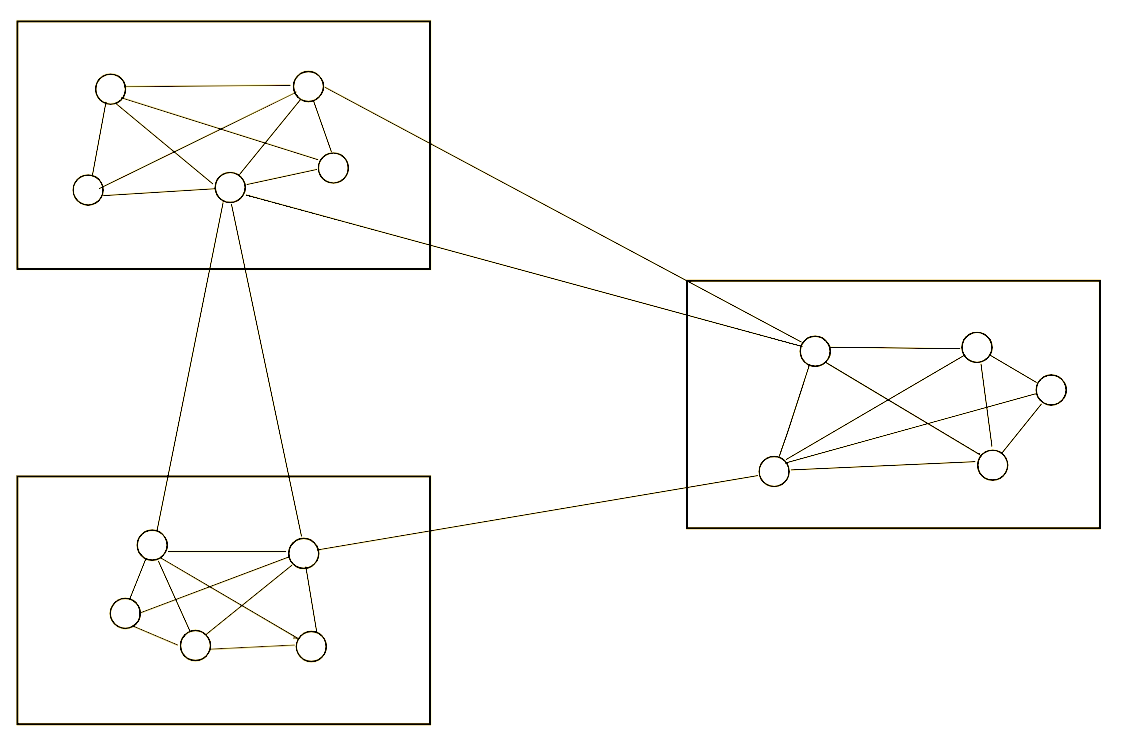
\includegraphics[width=0.48\textwidth]{assets/acba.png}}
  \hfill
  \subfloat[Forte accoppiamento]{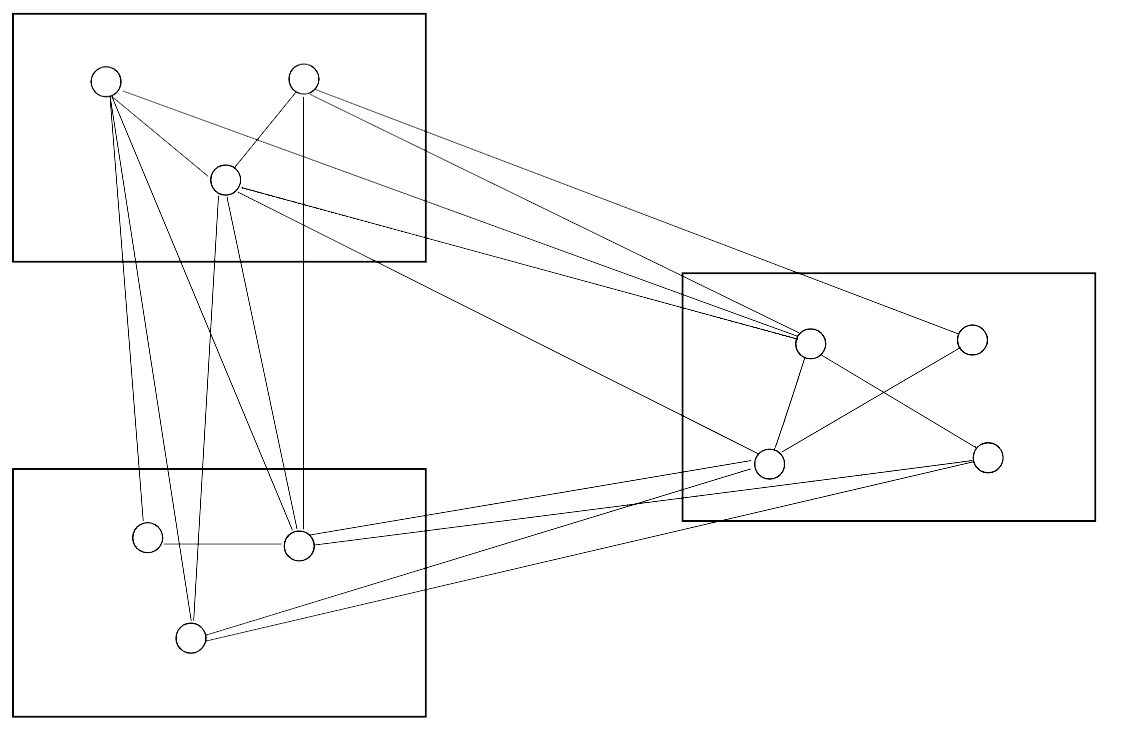
\includegraphics[width=0.48\textwidth]{assets/accopp.png}}
  \caption{Coesione e accoppiamento nei moduli}
\end{figure}

\section{Caso Studio - Compilatore}

Lo sviluppo di un compilatore segue metodi sistematici e formali di progettazione (spesso imposti da comitati - es. BNF, teoria degli automi). Applica i seguenti principi:
\begin{itemize}
    \item \textbf{Separazione deli interessi}, ci si concentra su efficienza e interfaccia.
    \item \textbf{Modularità}, il processo è scomposto in fasi: analisi lessicale, analisi sintattica (\textit{parsing}) e generazione di codice (intermedio $\rightarrow$ macchina)
    \item \textbf{Astrazione} tramite la generazione di codice intermedio (es. Java Bytecode)
    \item \textbf{Anticipazione del cambiamento} tramite l'utilizzo di librerie standard, ci si predispone a cambiamenti e/o estensioni.
    \item \textbf{Generalità} tramite codice intermedio per generalizzare (parametrizzare) l'architettura della macchina. La generazione stessa di compilatori è un processo automatizzato (tramite \textit{compiler compilers}).
    \item \textbf{Incrementalità} tramite versioning, permette: estensione della sintassi, migliori livelli di diagnostica, ottimizzazioni.
\end{itemize}

\begin{figure}
    \centering
    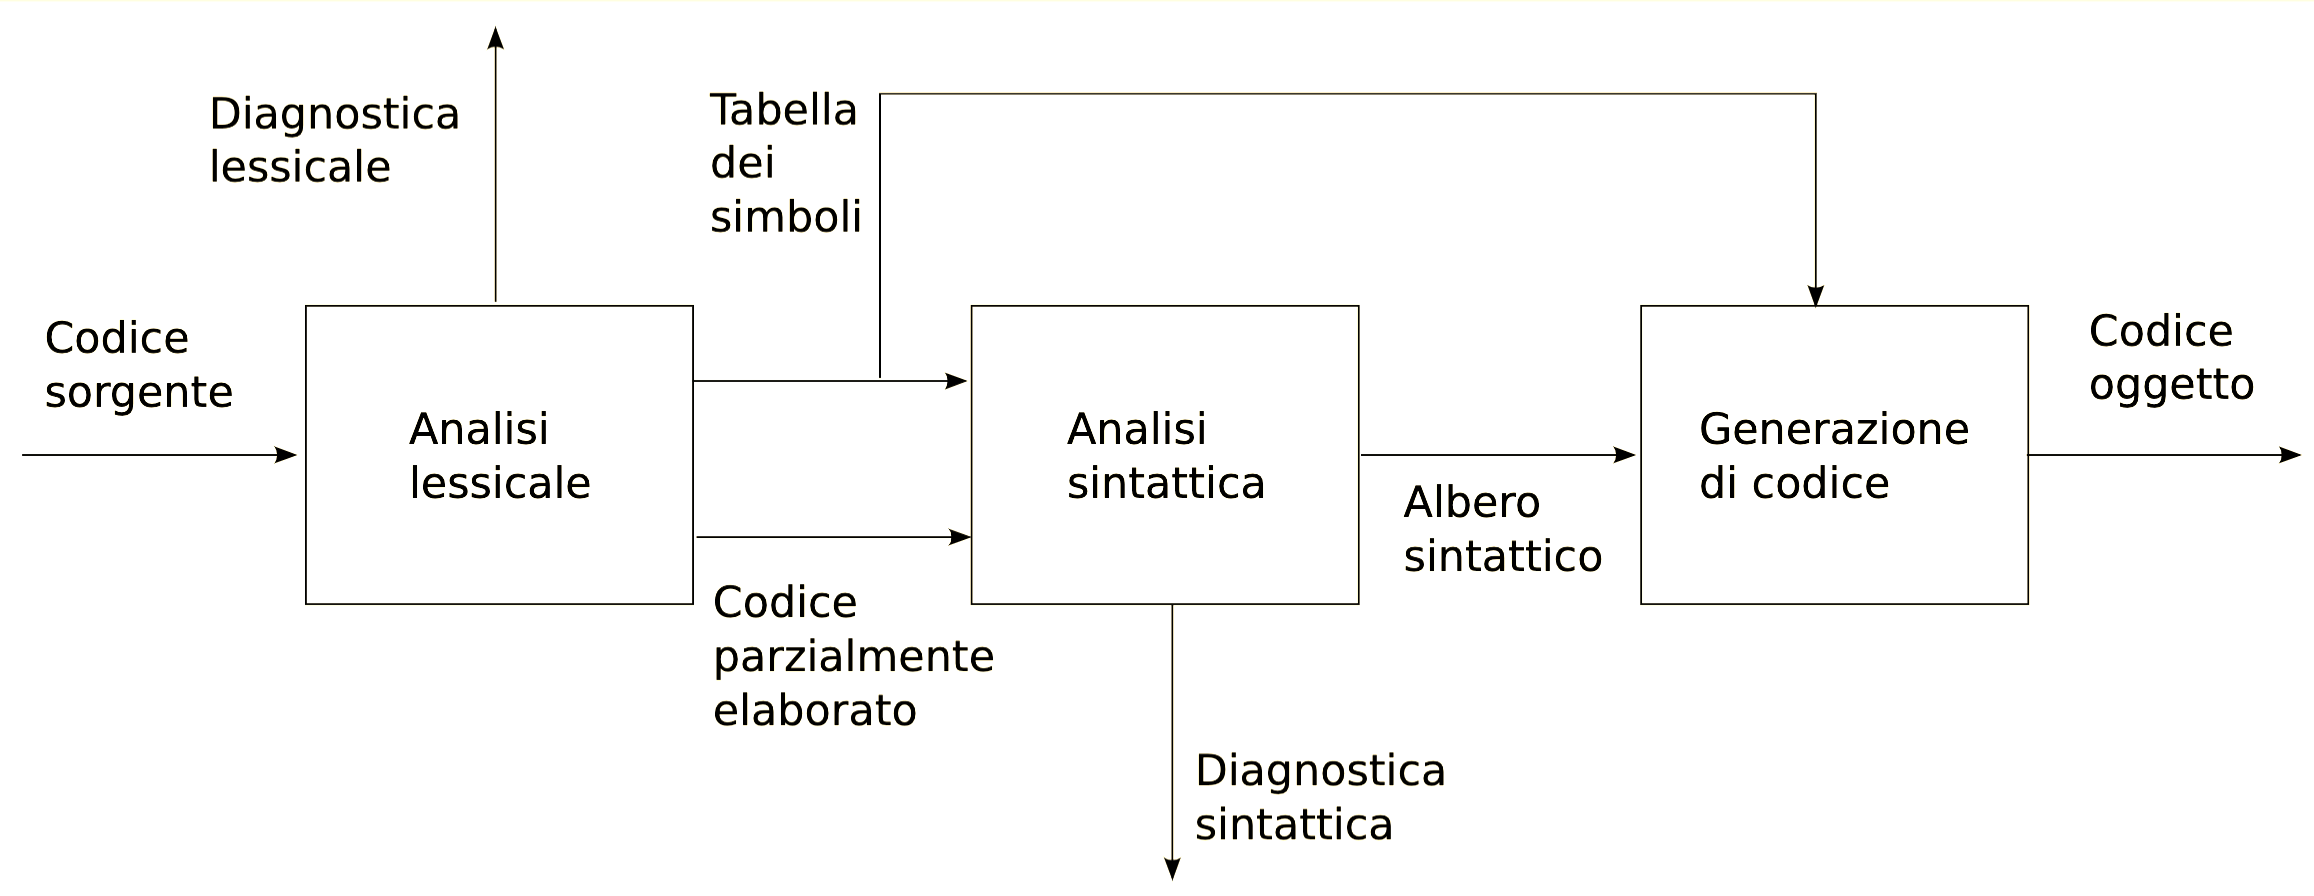
\includegraphics[width=1\linewidth]{assets/compilatore.png}
    \caption{Rappresentazione della struttura modulare del compilatore}
\end{figure}

\begin{figure}
    \centering
    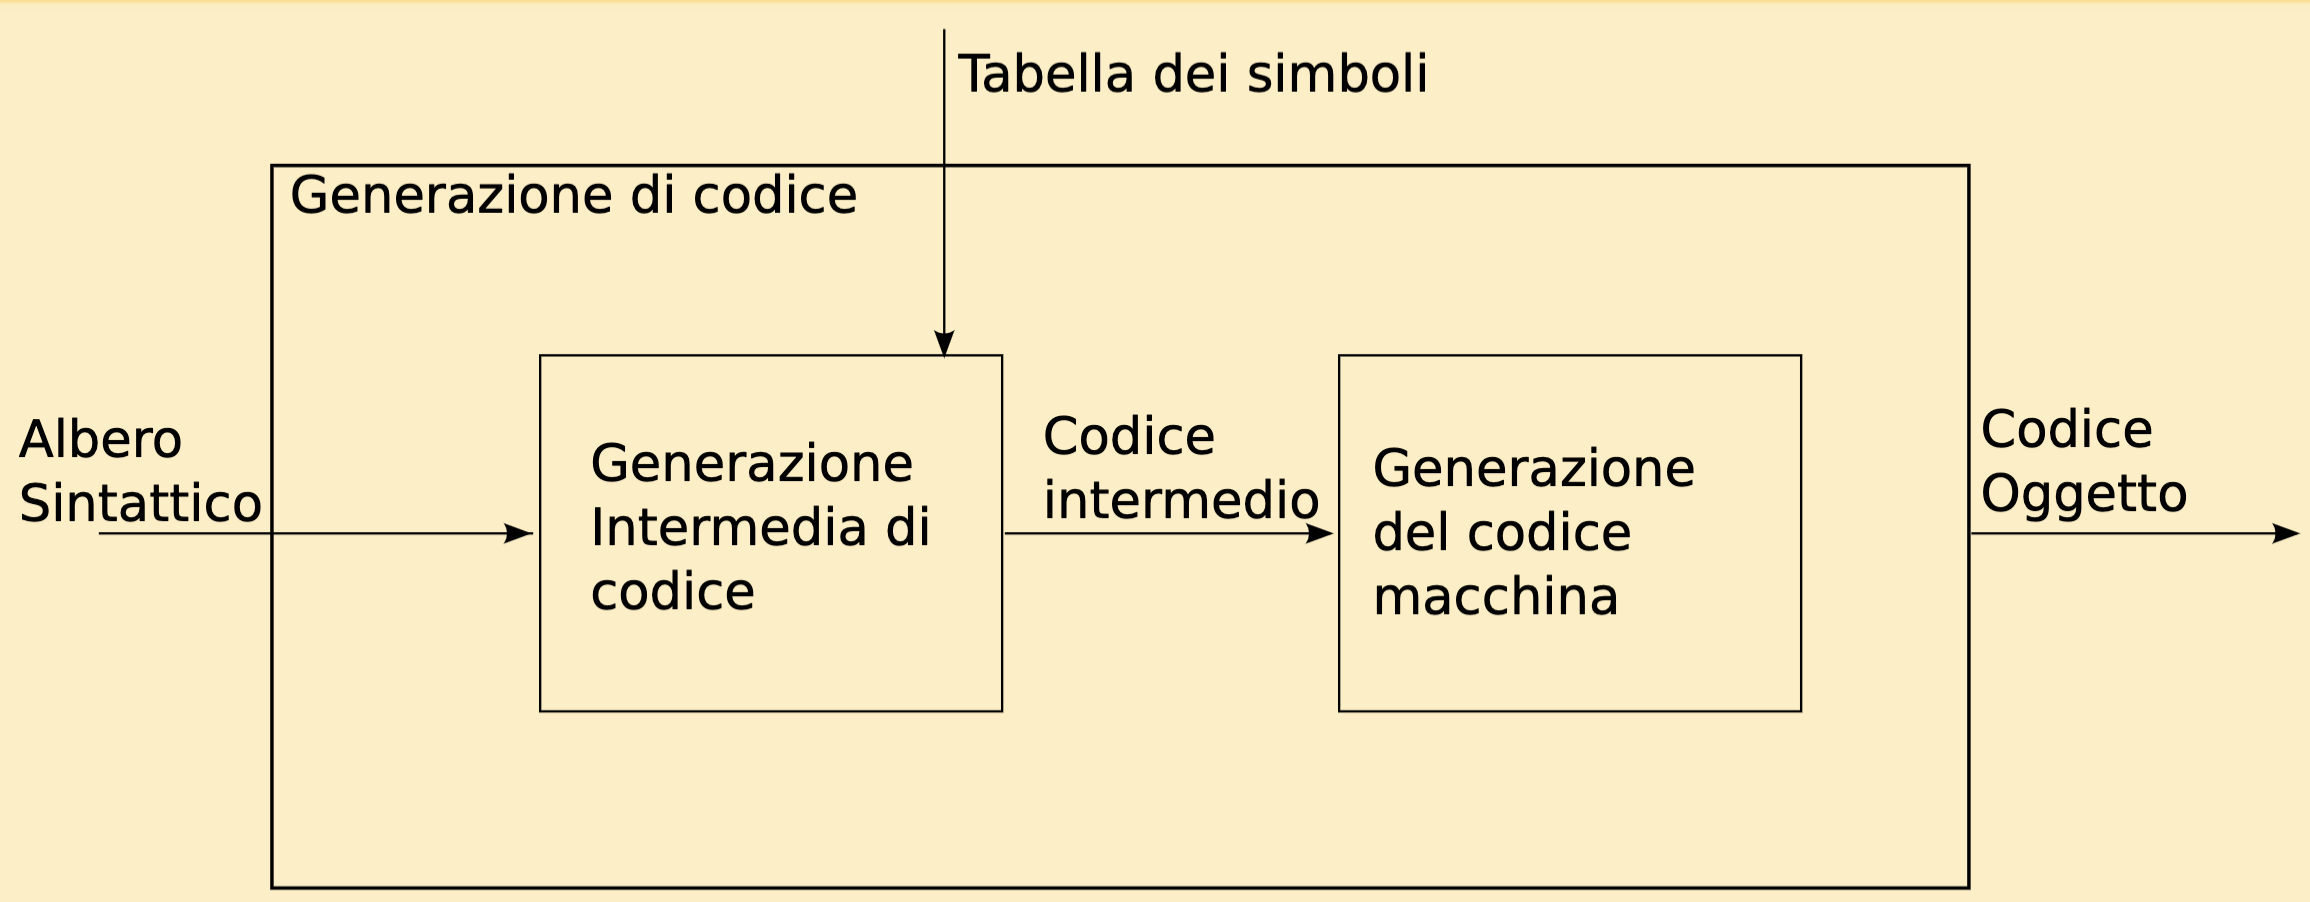
\includegraphics[width=1\linewidth]{assets/gencod.png}
    \caption{Ulteriore modularizzazione del modulo di generazione del codice}
\end{figure}

\newpage